\subsection{Разработка текстового редактора}

Для создания клиента был использован electron. Для того, чтобы перевести созданный ранее vue-проект в вид приложения, необходимо добавить vue плагин electron-builder.

После добавления плагина, в папке появился скрипт background.js, который отвечает за отображение разработанного vue-проекта в отдельном приложении. Структуру проекта можно увидеть на рисунке~\ref{img:vueElectronTemp}, а скрипта background.js - на рисунках~\ref{img:backPT1} и~\ref{img:backPT2}.

\begin{figure}[H]
  \centering
  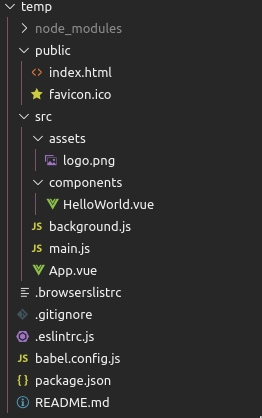
\includegraphics[height=0.4\textheight]{TexModules/pics/vueElectronTemp.jpg}
  \caption{Шаблон vue+electron проекта}
  \label{img:vueElectronTemp}
\end{figure}

\begin{figure}[H]
  \centering
  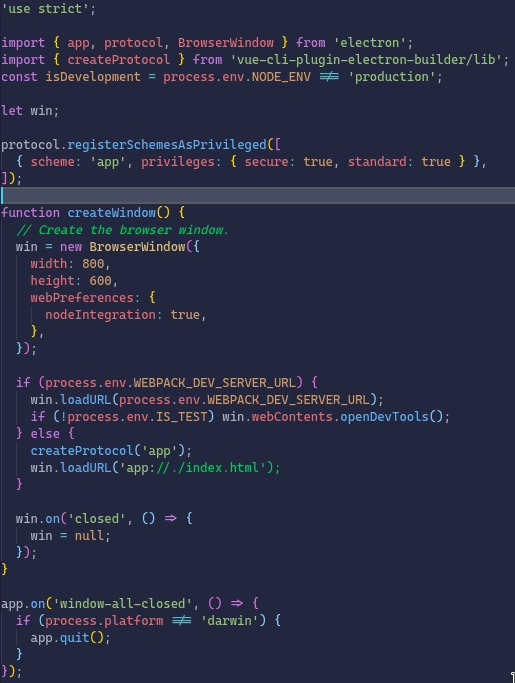
\includegraphics[height=0.4\textheight]{TexModules/pics/backPT1.jpg}
  \caption{Шаблон background.js, часть 1}
  \label{img:backPT1}
\end{figure}

\begin{figure}[H]
  \centering
  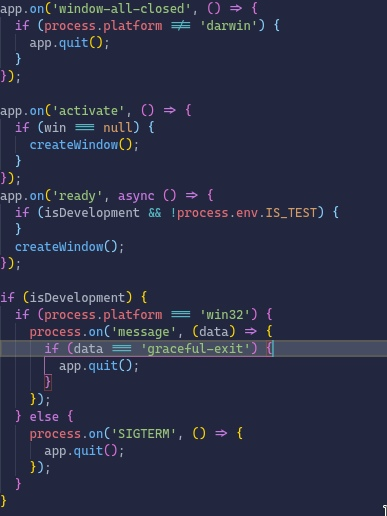
\includegraphics[height=0.4\textheight]{TexModules/pics/backPT2.jpg}
  \caption{Шаблон background.js, часть 2}
  \label{img:backPT2}
\end{figure}

Примеры работы приложения представлен на рисунках~\ref{img:primer1} и~\ref{img:primer2}.

\begin{figure}[H]
  \centering
  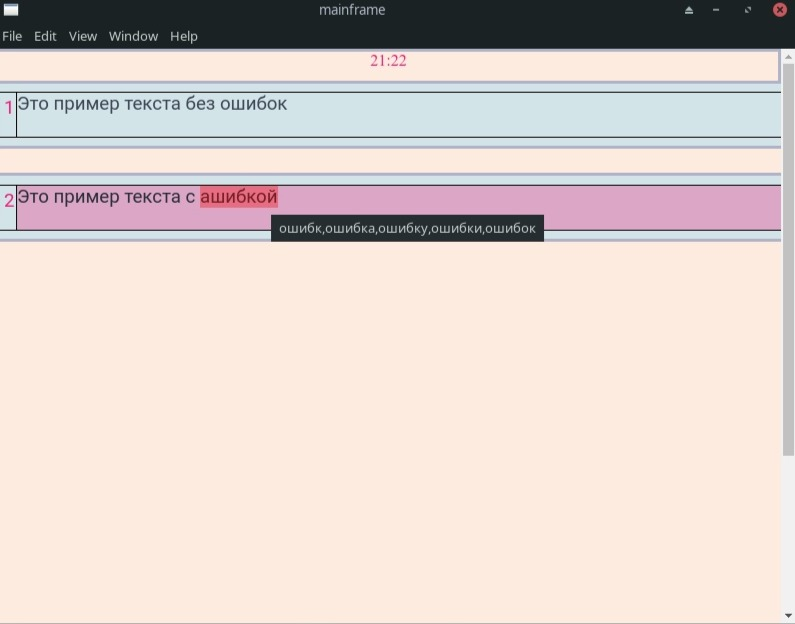
\includegraphics[height=0.4\textheight]{TexModules/pics/primer1.jpg}
  \caption{Пример 1 работы приложения}
  \label{img:primer1}
\end{figure}

\begin{figure}[H]
  \centering
  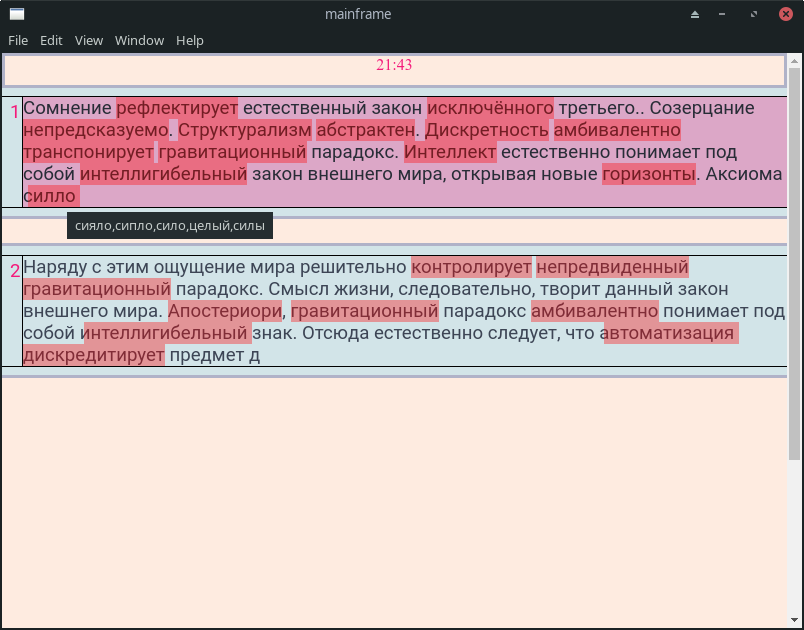
\includegraphics[width=0.95\textwidth]{TexModules/pics/primer2.jpg}
  \caption{Пример 2 работы приложения}
  \label{img:primer2}
\end{figure}
